\Subhead{2.7.2}{Дифракция в зоне Френеля и Фраунгофера. Характеристики поля в фокусе линзы}

Для параксиального распространения от плоскости $z=0$ разлагают расстояние $R\simeq z+[(x-x')^2+(y-y')^2]/(2z)$. Скалярное поле приближённо равно
\begin{equation}
 U(x,y,z)=\frac{\e^{\ii kz}}{\ii\lambda z}\iint U(x',y',0)
 \exp\left\{\frac{\ii k}{2z}[(x-x')^2+(y-y')^2]\right\}\dd x'\dd y'.
\end{equation}
Число Френеля $N_F=a^2/(\lambda z)$ сравнивает квадратичную фазу на апертуре с единицей. В зоне Фраунгофера $N_F\ll1$ квадратичной фазой по координатам источника пренебрегают; поле пропорционально преобразованию Фурье апертуры при $k_x=kx/z$, $k_y=ky/z$. Для равномерной щели ширины $a$ интенсивность имеет вид $I\propto\operatorname{sinc}^2(ka\sin\theta/2)$, где $\operatorname{sinc}x=\sin x/x$.

Тонкая линза вносит фазу $-kr'^2/(2f)$, компенсирующую квадратичную фазу распространения в заднюю фокальную плоскость. Поэтому там получается угловой спектр падающего поля. Для круглой равномерно освещённой апертуры диаметра $D$
\begin{equation}
 \frac{I(r)}{I(0)}=\left[\frac{2J_1(\xi)}{\xi}\right]^2,
 \quad \xi=\frac{\pi Dr}{\lambda f},\quad
 r_{\rm first}=1.22\frac{\lambda f}{D}.
\end{equation}
Это пятно Эйри. Первый нуль и ширина по половине максимума — разные характеристики. Уменьшение апертуры увеличивает пятно; аберрации и неоднородное освещение меняют профиль. Фокус — не геометрическая точка, а дифракционная область.
\begin{center}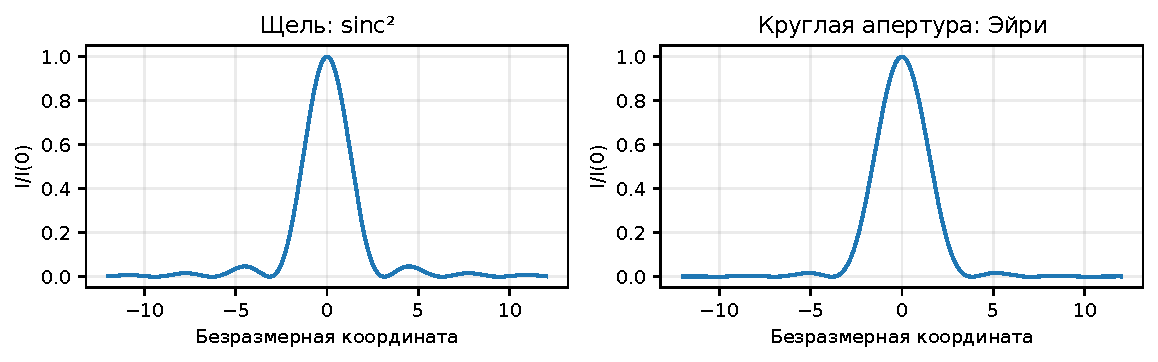
\includegraphics[width=0.82\linewidth]{figures/diffraction.pdf}\end{center}

